\documentclass[10pt,twocolumn,letterpaper]{article}
\usepackage[T1]{fontenc}
\usepackage[pagenumbers]{cvpr}
\usepackage{microtype}
\definecolor{cvprblue}{rgb}{0.16,0.30,0.50}
\usepackage[breaklinks,colorlinks,allcolors=cvprblue]{hyperref}
\graphicspath{{../results/metric-research/figures/}{../results/figures/}{../results/metric-research/}}
\newcommand{\NyuAbsRel}{0.11455}
\newcommand{\NyuRMSE}{0.39889}
\newcommand{\NyuDelta}{0.89222}
\newcommand{\StereoMAE}{1.895}
\newcommand{\StereoCoverage}{75.69}
\newcommand{\TemporalGain}{18.23}
\newcommand{\EdgeRetention}{97.58}
\newcommand{\OriginalFPS}{2.77}
\newcommand{\EfficientFPS}{4.34}
\newcommand{\SpeedGain}{56.9}
\newcommand{\EfficientGain}{16.82}
\newcommand{\EfficientEdge}{97.64}

\newcommand{\ResearchMethod}{rank-8 Q/V LoRA with fixed flip averaging}
\newcommand{\ResearchBaseAbs}{0.11455}
\newcommand{\ResearchFinalAbs}{0.08112}
\newcommand{\ResearchGain}{29.18}
\newcommand{\ResearchPreviousGain}{15.19}
\newcommand{\ResearchGainCI}{[25.93, 32.41]\%}
\newcommand{\ResearchImproved}{486}
\newcommand{\ResearchWorsened}{168}
\newcommand{\ResearchRefitComparison}{AbsRel decreases by 1.44\% after the all-development refit}
\newcommand{\ResearchSeeds}{320112, 320113, 320114}
\newcommand{\ResearchBaseMS}{37.4}
\newcommand{\ResearchFinalMS}{235.8}

\def\confName{CVPR}
\def\confYear{2027}
\title{Data-Efficient Adaptation of Small-Model Metric Depth\\with Scene-Separated Selection and Frozen Evaluation}
\author{Eugene\\HKUST (Guangzhou)\\AIAA 3201 Computer Vision Project}
\begin{document}
\maketitle
\begin{abstract}
We reproduce the course's UniDepthV2 ViT-S metric-depth reference and investigate lightweight improvements using the permitted NYU development split. A controlled search compares residual refinement, native-feature conditioning, image-dependent calibration, input resolution, and low-rank internal adaptation. Whole-scene cross-validation and three training seeds select \ResearchMethod{}. The final model is refitted on all 795 development images for a duration fixed from cross-validation. On all 654 test images, AbsRel changes from \ResearchBaseAbs{} to \ResearchFinalAbs{}, a \ResearchGain\% reduction. Against our previously completed residual refiner, the reduction is \ResearchPreviousGain\%. These measurements use RGB-only inference and the same raw-metric evaluation support. Development supervision and additional inference cost are stated explicitly. We retain per-image regressions and show shared-scale depth, ground-truth error, runtime, and a depth-based application. The mandatory 15-pair stereo exercise and relative DA V2/VDA comparison are also included. The linked video supplies 70 genuine frames. Code and results are available at \url{https://github.com/Lingxiaolingqc/MMDEVC/tree/experiment/independent-metric-optimization-20261113/independent}.
\end{abstract}

\section{Introduction}
Suppose a table is 2 m from the camera. Predicting 1.6 m gives proportional error $|1.6-2|/2=0.2$. Multiplying every prediction by 1.25 fixes this simplified example. It also moves a correctly predicted 4 m wall to 5 m. This illustrates why useful refinement must be tested against measured distances across held-out scenes.

Our research question is whether limited labeled development data can adapt a pretrained Small model to indoor metric depth through a small trainable parameter set and controlled prediction averaging. We examine global distance bias, domain-specific prediction errors, and variation across views and training runs.

The assignment names UniDepthV2 and Depth Pro as single-image metric references and Video Depth Anything as the video reference. We select UniDepthV2 ViT-S for quantitative improvement. Its pretrained checkpoint predicts distances in meters from RGB. NYU supplies the target depth labels used for development adaptation and final evaluation. We preserve the original reference prediction and compare every method with the same crop, valid-depth mask, units, and aggregation.

Our initial residual refinement already reduced test AbsRel by 16.50\%. The present study preserves that result and asks whether limited development data can support a stronger method. We first measure how performance changes with the number of fitting scenes. We then compare interventions at calibration, output refinement, frozen representation, internal adaptation, and input resolution. Selection uses development evidence before the final weights and recipe are frozen.

The final comparison addresses this course reference under a stated supervised-adaptation setting. A broader state-of-the-art claim would require matched comparisons with other methods, training data, preprocessing, and evaluation protocols. Our evidence consists of the reproduced reference, the previous completed method, and the new frozen model on the same 654 NYU images.

\section{Related Work}
Semi-global matching~\cite{hirschmuller2008} connects image correspondence to calibrated stereo depth, and Middlebury~\cite{scharstein2014} provides detailed disparity ground truth. NYU~\cite{silberman2012} supplies indoor RGB-D evaluation. KITTI~\cite{geiger2012} and TUM RGB-D~\cite{sturm2012} illustrate other scene and sensor distributions.

DPT~\cite{ranftl2021} develops transformer-based dense prediction. Depth Anything and DA V2~\cite{yang2024da,yang2024dav2} learn transferable relative-depth representations. UniDepth and UniDepthV2~\cite{piccinelli2024,piccinelli2025} estimate metric geometry with camera-aware prediction. Depth Pro~\cite{bochkovskii2025} is the assignment's alternative metric model. Video Depth Anything~\cite{chen2025} uses temporal modeling to improve long-video depth consistency.

RAFT~\cite{teed2020} supports the brief's flow-guided fusion direction. Guided filtering~\cite{he2010guided} motivates image-guided output processing, while encoder--decoder skip connections~\cite{ronneberger2015unet} motivate the small residual refiner. LoRA~\cite{hu2022lora} adapts a pretrained network through low-rank weight updates. We use standard Q/V LoRA as a competing lightweight technique, evaluated through the official UniDepthV2 RGB-only path.

\section{Data and Evaluation}
\subsection{Ground Truth and Partitions}
The official labeled NYU set contains 1,449 RGB-D pairs. Its split assigns 795 images to development and 654 to testing. We initially divide development into 577 fitting images from 187 scenes and 218 selection images from 62 different scenes. The test split contains 215 scenes. The 218 images select methods and seeds before the all-development refit. Their earlier scores measure pre-refit selection performance.

Within the 577-image fitting pool, three whole-scene folds use fitting/held-out counts of 390/187, 373/204, and 391/186. Every fold refits label-dependent calibration on its own fitting portion. The final refit uses all 795 development images with no validation subset and a fixed duration. No test labels enter calibration, checkpoint selection, seed selection, or refitting.

The labeled MAT file was obtained through a public mirror. Its first MiB matched the official endpoint, and the complete local SHA-256 is recorded. An independently published official full-file checksum was unavailable. The dataset, official split, model checkpoint, source revisions, and prediction identities are retained in machine-readable records.

\subsection{Common NYU Protocol}
We evaluate at $480\times640$ with crop $[45:471,41:601]$. Ground truth must be finite and strictly between 0.001 and 10 m. Predictions are clipped to $[0.001,10]$ m. Nonfinite outputs fail evaluation. AbsRel is mean $|p-g|/g$, RMSE is the square root of mean squared error in meters, and $\delta_1$ is the fraction with $\max(p/g,g/p)<1.25$. Each image receives equal weight.

AbsRel determines selection. RMSE and $\delta_1$ remain reported because a method can change different error characteristics. Test predictions use RGB and frozen model parameters. A separate scoring pass reads ground truth from saved float predictions. It applies no per-test scale alignment.

We report 5,000-replicate paired scene-cluster bootstrap intervals, which resample entire scenes. These intervals condition on the fitted models and omit the uncertainty introduced by the search itself. Three-seed standard deviations describe the measured variation between training runs.

\subsection{Other Required Inputs}
Stereo uses all 15 Middlebury quarter-resolution pairs with their calibration and \texttt{disp0GT.pfm}. The official archive uses the folder name \texttt{trainingQ}. The linked rollercoaster video decodes to 70 genuine frames at $960\times540$, 24 FPS. Both relative models process exactly those frames and display $640\times360$ outputs. The source cannot supply frames 70--99. The archive records the actual count.

\section{Competing Lightweight Methods}
\subsection{Calibration and Residual Refinement}
The official pretrained UniDepthV2 ViT-S is the raw metric reference. Default preprocessing rounds NYU input to an internal $490\times644$. Original and horizontally flipped RGB predictions are restored to matching coordinates. The previous method uses a fixed 0.25 flip weight, development-fitted scale 0.9413383, and a 388,001-parameter residual network.

The refiner consumes RGB, log original/flip/base depth, transformed model confidence, and normalized coordinates at $240\times320$. It predicts bounded log corrections applied multiplicatively to the base map. Encoder widths are 16, 32, 64, and 96 with skip-connected bilinear decoding. We retain the previous weights and use an explicit control trainer for the new study.

New candidates test RGB augmentation, dropout, narrower layers, full-resolution supervision, and a log-depth gradient loss. Native-feature variants add 256-channel frozen depth features through a learned projection, with an optional gate. A wider residual bound is another ablation. These interventions share the same test-time information available from RGB and the foundation model.

An additional ridge-regression candidate predicts an image-specific log scale from 256 globally pooled native features and seven log-depth statistics. Its regularization is chosen in fitting-scene folds. This follows the metric-calibration motivation while allowing the multiplier to depend on the image.

\subsection{Limited Internal Adaptation}
LoRA preserves a pretrained weight matrix $W$ and learns two smaller matrices,
\begin{equation}
W'=W+BA, \quad A\in\mathbb{R}^{r\times d},\quad B\in\mathbb{R}^{d\times r}.
\end{equation}
The input RGB is independent of these learned parameters. The prediction is the resulting metric-depth map, and NYU depth is the training target. Initializing $B$ to zero makes the initial prediction exactly match the pretrained model.

We add independent updates to the query and value projections in each of the 12 ViT-S blocks. Rank 4 trains 73,728 parameters and rank 8 trains 147,456. Pretrained attention weights, keys, normalization, camera prediction, and decoder parameters remain frozen. Frozen tensor digests are checked before and after training. The official model stays in evaluation mode while gradients update the adapters.

Training uses the official differentiable RGB-only preprocessing and geometry, a fitting-only global scale, full-resolution course-protocol AbsRel, AdamW, FP16 scaling, and gradient clipping at 1. An effective batch of 8 is accumulated through microbatches of 2. The learning-rate schedule has an 80-epoch horizon. Scene-fold and repeated-seed runs allow at most 80 epochs with patience 20 after epoch 24.

A fixed 0.25 restored-flip average is evaluated as an inference variant. A fixed equal prediction mean with the best feature refiner is another declared contender. Their trained component weights are reused. New weights are trained for each fitting-scene partition, and validation labels select among the resulting candidates.

\begin{figure*}[t]
\centering
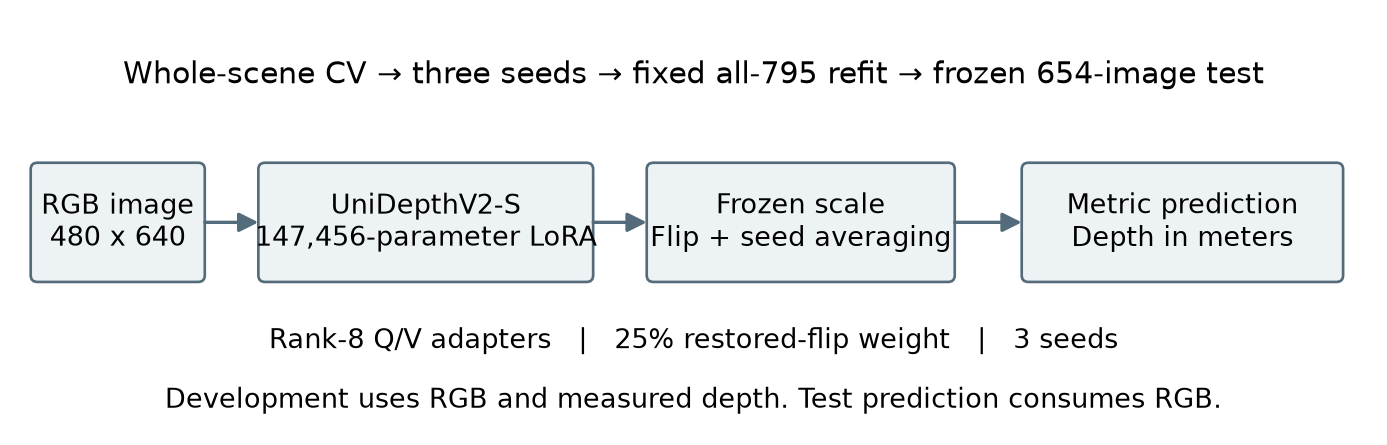
\includegraphics[width=\textwidth]{research-pipeline.png}
\caption{Development selection and final RGB-only inference. Ground-truth labels fit calibration and lightweight parameters during development. The frozen test path consumes RGB. The selected recipe and all-development weights are recorded before test predictions are generated.}
\label{fig:pipeline}
\end{figure*}

\subsection{Data Efficiency and Selection}
The data-size study uses three seeds and nested whole-scene subsets near 100, 200, 400, and 577 images. Every run has the same maximum update budget. Mean selection AbsRel is 0.10840, 0.10676, 0.10305, and 0.10305. For this architecture, increasing from about 400 to 577 images supplies no demonstrated additional gain. This motivates improving how pretrained representations are adapted.

\begin{figure*}[t]
\centering
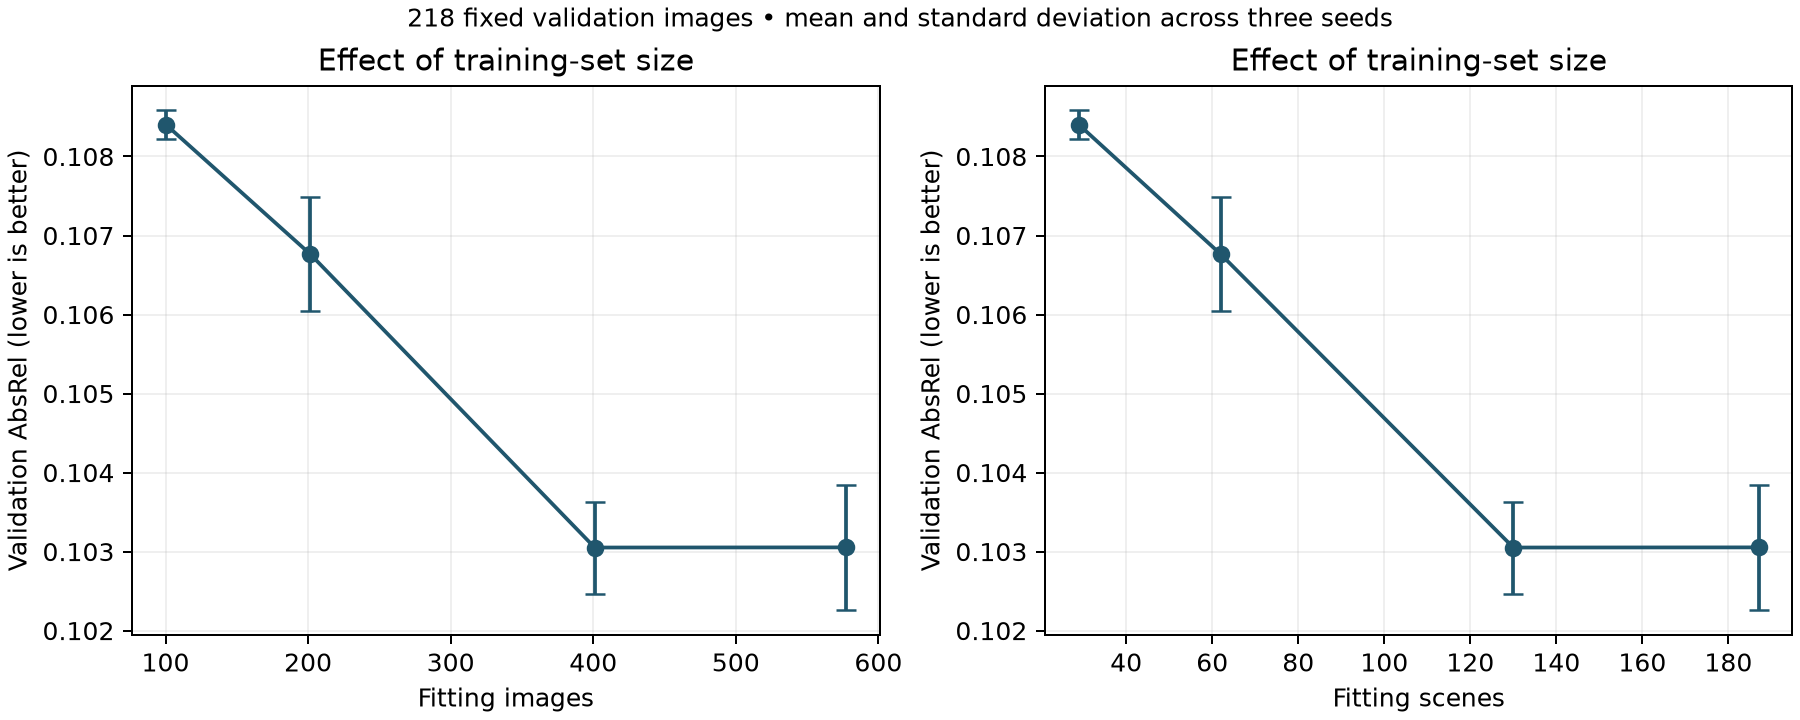
\includegraphics[width=.95\textwidth]{learning-curves.png}
\caption{Fixed 218-image selection split. Each point averages three seeds, with standard deviation shown. Image counts and distinct scene counts are both retained. The result concerns the residual-refiner family used in this study.}
\label{fig:curves}
\end{figure*}

The first pilot stage establishes which families warrant scene-fold evaluation. The plain control reaches selection AbsRel 0.10189. The best gated native-feature refiner reaches 0.09226. Image-dependent ridge calibration reaches 0.09662. Rank-8 LoRA reaches 0.08629, and its fixed flip variant reaches 0.08504. These pilot scores guide further development comparisons.

Larger-input studies use actual internal sizes $532\times700$ and $658\times868$. Their globally calibrated selection errors are 0.10773 and 0.10871, compared with 0.10843 at the default resolution. Higher resolution therefore supplies no substantial gain over the stronger adaptation candidates in this study.

\begin{table}[t]
\centering\small
\caption{Equal means over three fitting-scene folds. Refit durations use median best fold epochs. Combined rows list LoRA/refiner durations.}
\begin{tabular}{lrr}
\toprule
Candidate & Mean AbsRel & Epochs\\
\midrule
LoRA/feature mean, high LR & 0.08652 & 19/40\\
LoRA/feature mean, low LR & 0.08739 & 18/40\\
LoRA + flip, LR $10^{-4}$ & 0.08792 & 19\\
LoRA, LR $10^{-4}$ & 0.08845 & 19\\
LoRA + flip, LR $3\times10^{-5}$ & 0.08935 & 18\\
LoRA, LR $3\times10^{-5}$ & 0.08970 & 18\\
Native features + gate & 0.09075 & 40\\
RGB residual control & 0.09817 & 28\\
\bottomrule
\end{tabular}
\end{table}

\begin{table}[t]
\centering\small
\caption{Three-seed selection results on the same 218 development images. SD describes training-seed variability.}
\begin{tabular}{lrr}
\toprule
Candidate & Mean AbsRel & SD\\
\midrule
RGB residual control & 0.10221 & 0.00059\\
LoRA + flip, LR $10^{-4}$ & 0.08630 & 0.00158\\
LoRA/feature mean, high LR & 0.08734 & 0.00102\\
LoRA, LR $10^{-4}$ & 0.08740 & 0.00156\\
LoRA + flip, LR $3\times10^{-5}$ & 0.08757 & 0.00077\\
LoRA/feature mean, low LR & 0.08818 & 0.00076\\
LoRA, LR $3\times10^{-5}$ & 0.08890 & 0.00076\\
Native features + gate & 0.09336 & 0.00090\\
\bottomrule
\end{tabular}
\end{table}



The two lowest mean-AbsRel configurations across all three scene folds advance to three seeds on the 577/218 partition. After these training runs, we evaluate all raw, flip-averaged, and combined inference variants sharing the trained weights. This expanded comparison is recorded before any new test metrics are inspected. Family selection uses mean seed error. Within the winning family, we compare the median-scoring single seed with the equal three-seed prediction average. We use the average only when its selection error is strictly lower. The final seed set is \ResearchSeeds{}, and the chosen family is \ResearchMethod{}. Each selected seed uses 147,456 learned rank-8 LoRA parameters. Each prediction blends 75\% original-view depth and 25\% restored-flip depth, followed by an equal average over three seeds. The fixed all-development refit duration is 19 epochs. The selected three-seed prediction mean reaches development AbsRel 0.08525.

The final fitting duration is the median best epoch from the three scene folds, rounded half up. It is fixed before the all-795 refit and uses the same 80-epoch schedule horizon. We predeclare the all-development model as final regardless of its later ordering against the pre-refit model on test.

\section{Results}
\subsection{Frozen Metric Comparison}
\begin{table}[t]
\centering\small
\caption{Complete 654-image NYU test comparison. Lower AbsRel/RMSE and higher $\delta_1$ are better.}
\begin{tabular}{lrrr}
\toprule
Method & AbsRel & RMSE (m) & $\delta_1$\\
\midrule
Raw UniDepthV2-S & 0.11455 & 0.39889 & 0.89222\\
Previous residual refiner & 0.09564 & 0.37080 & 0.91374\\
Selected (577 fit) & 0.08231 & 0.33517 & 0.93979\\
Final (795 fit) & 0.08112 & 0.33135 & 0.94236\\
\bottomrule
\end{tabular}
\end{table}

All four methods share the same 654 test images and evaluation arithmetic. The raw foundation is the course-named reference. The previous method uses its preserved weights. The pre-refit model uses the selected 577-image checkpoint(s), while the final model uses the complete 795-image development refit.

The final AbsRel reduction relative to the raw reference is \ResearchGain\%, with paired-scene 95\% interval \ResearchGainCI{}. Against the previous residual refiner, the reduction is \ResearchPreviousGain\%. The final model improves \ResearchImproved{} images and worsens \ResearchWorsened{} relative to the raw reference. In the pre-refit/full-refit comparison, \ResearchRefitComparison{}.

\begin{figure*}[t]
\centering
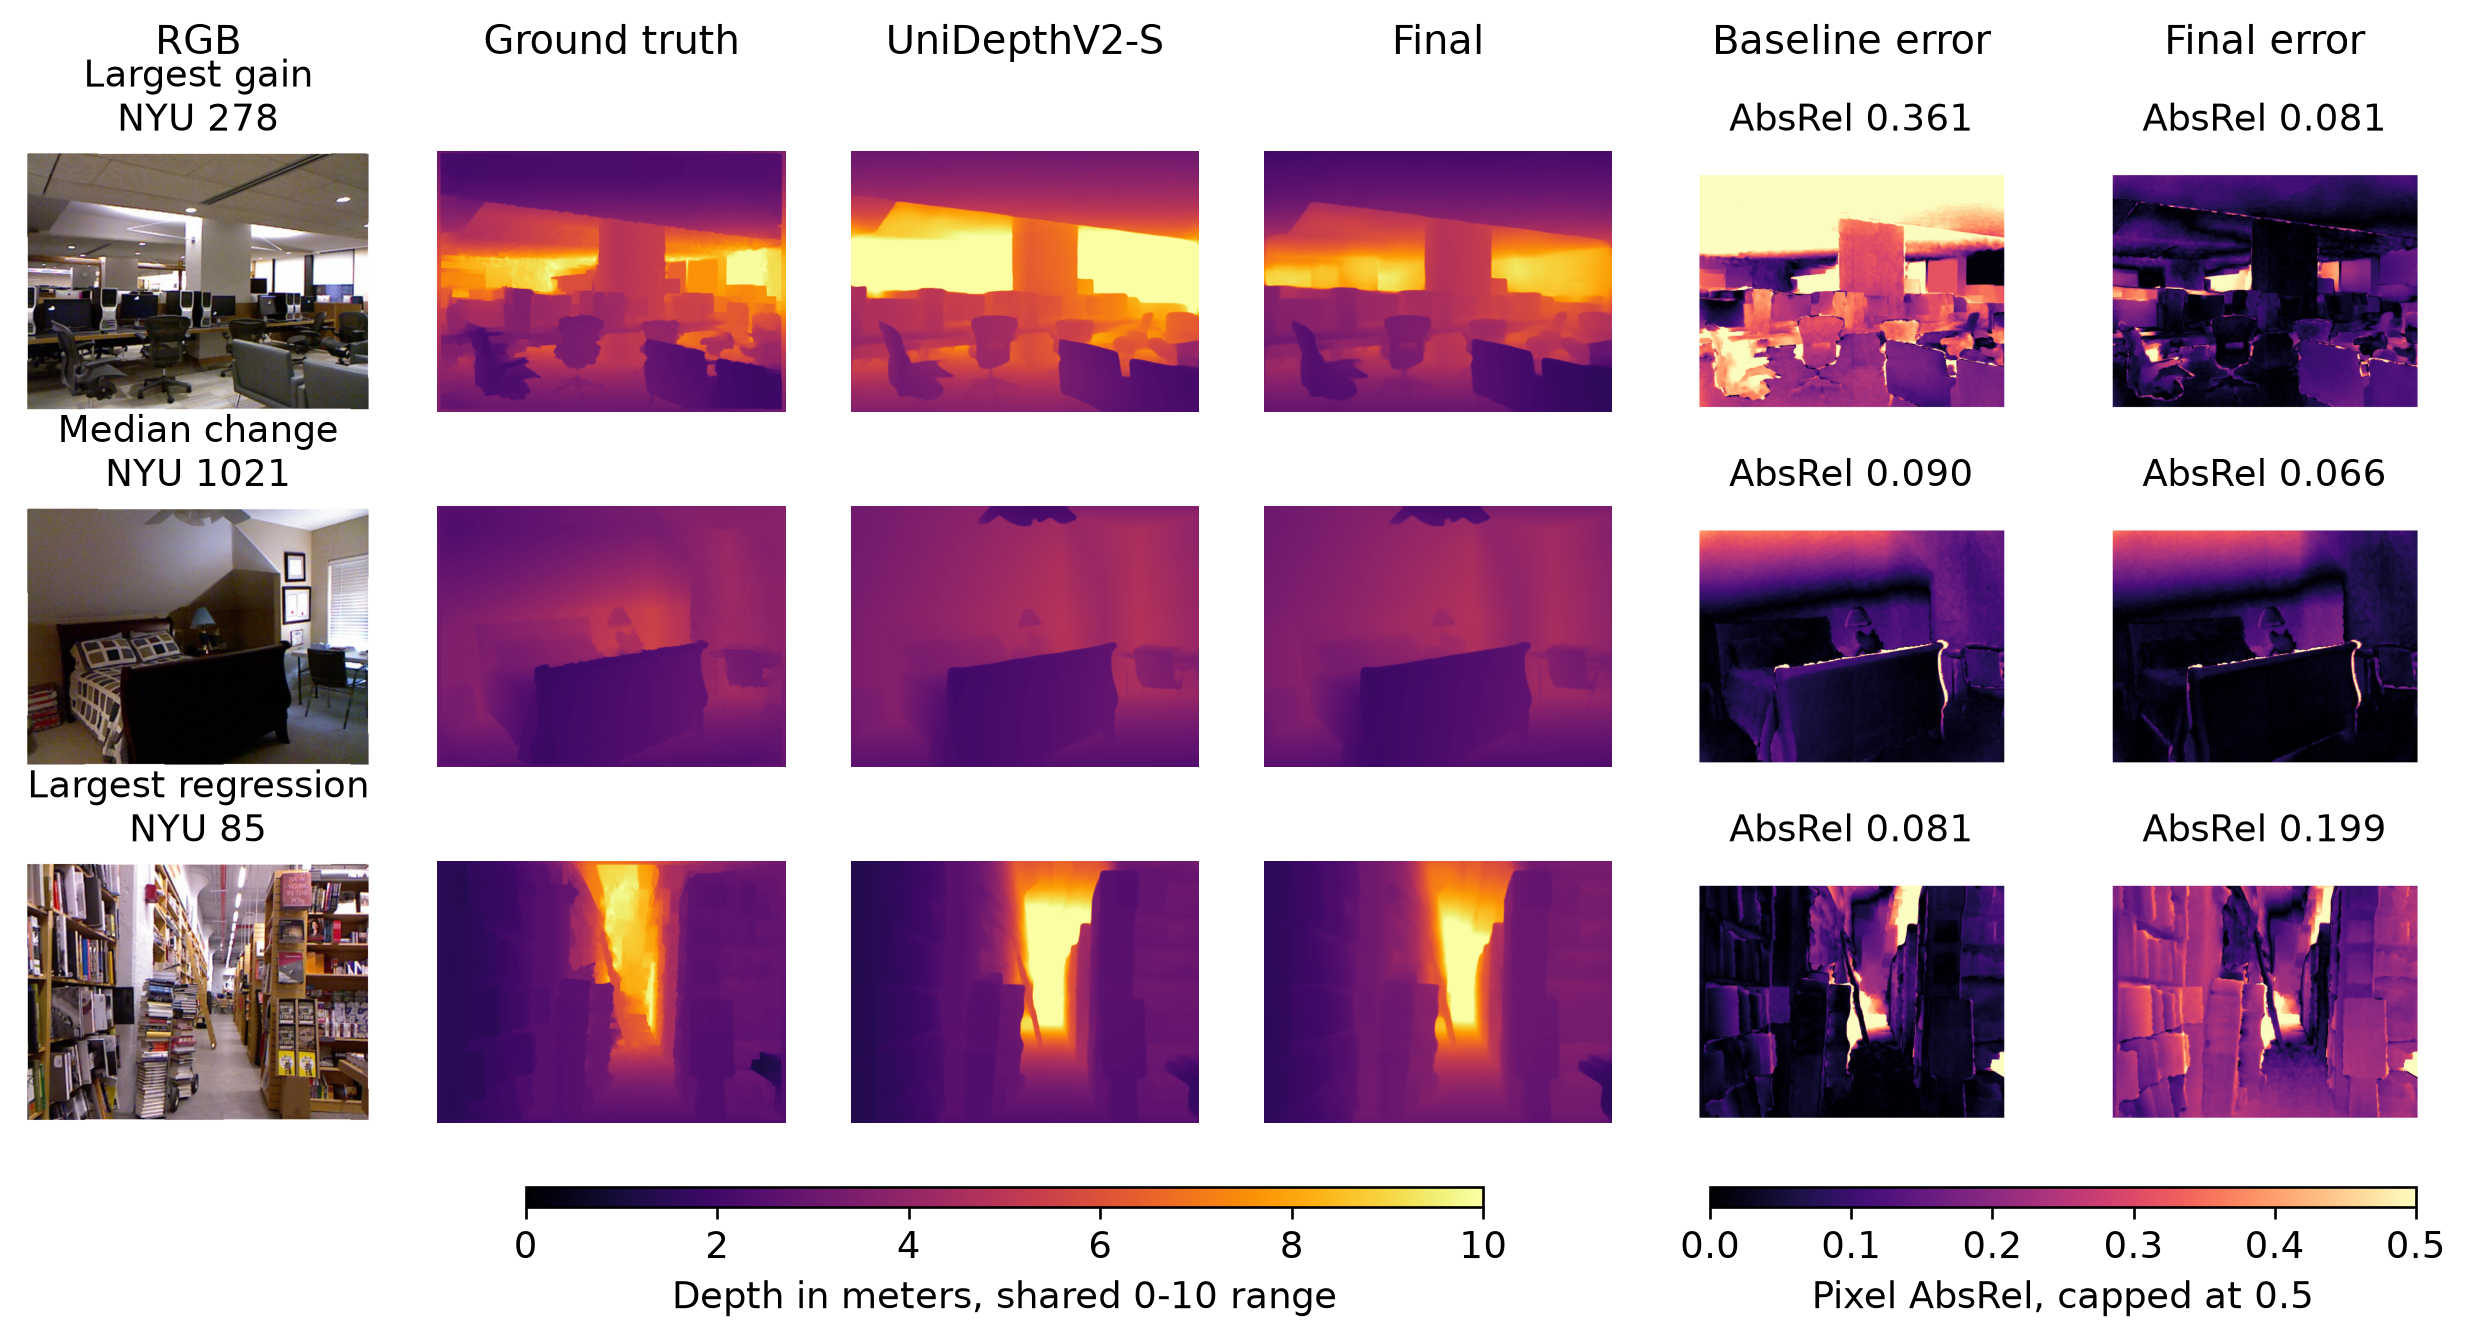
\includegraphics[width=\textwidth]{research-comparison.png}
\caption{RGB, measured depth, raw reference, and selected improvement with common 0--10 m colors. Ground-truth error maps share a fixed scale, with darker pixels indicating smaller errors. Rows follow the declared largest gain, median change, and largest regression selection rule. Per-image scores expose differences that can be hard to see in colored depth alone.}
\label{fig:comparison}
\end{figure*}

\subsection{Failure Analysis}
\begin{figure*}[t]
\centering
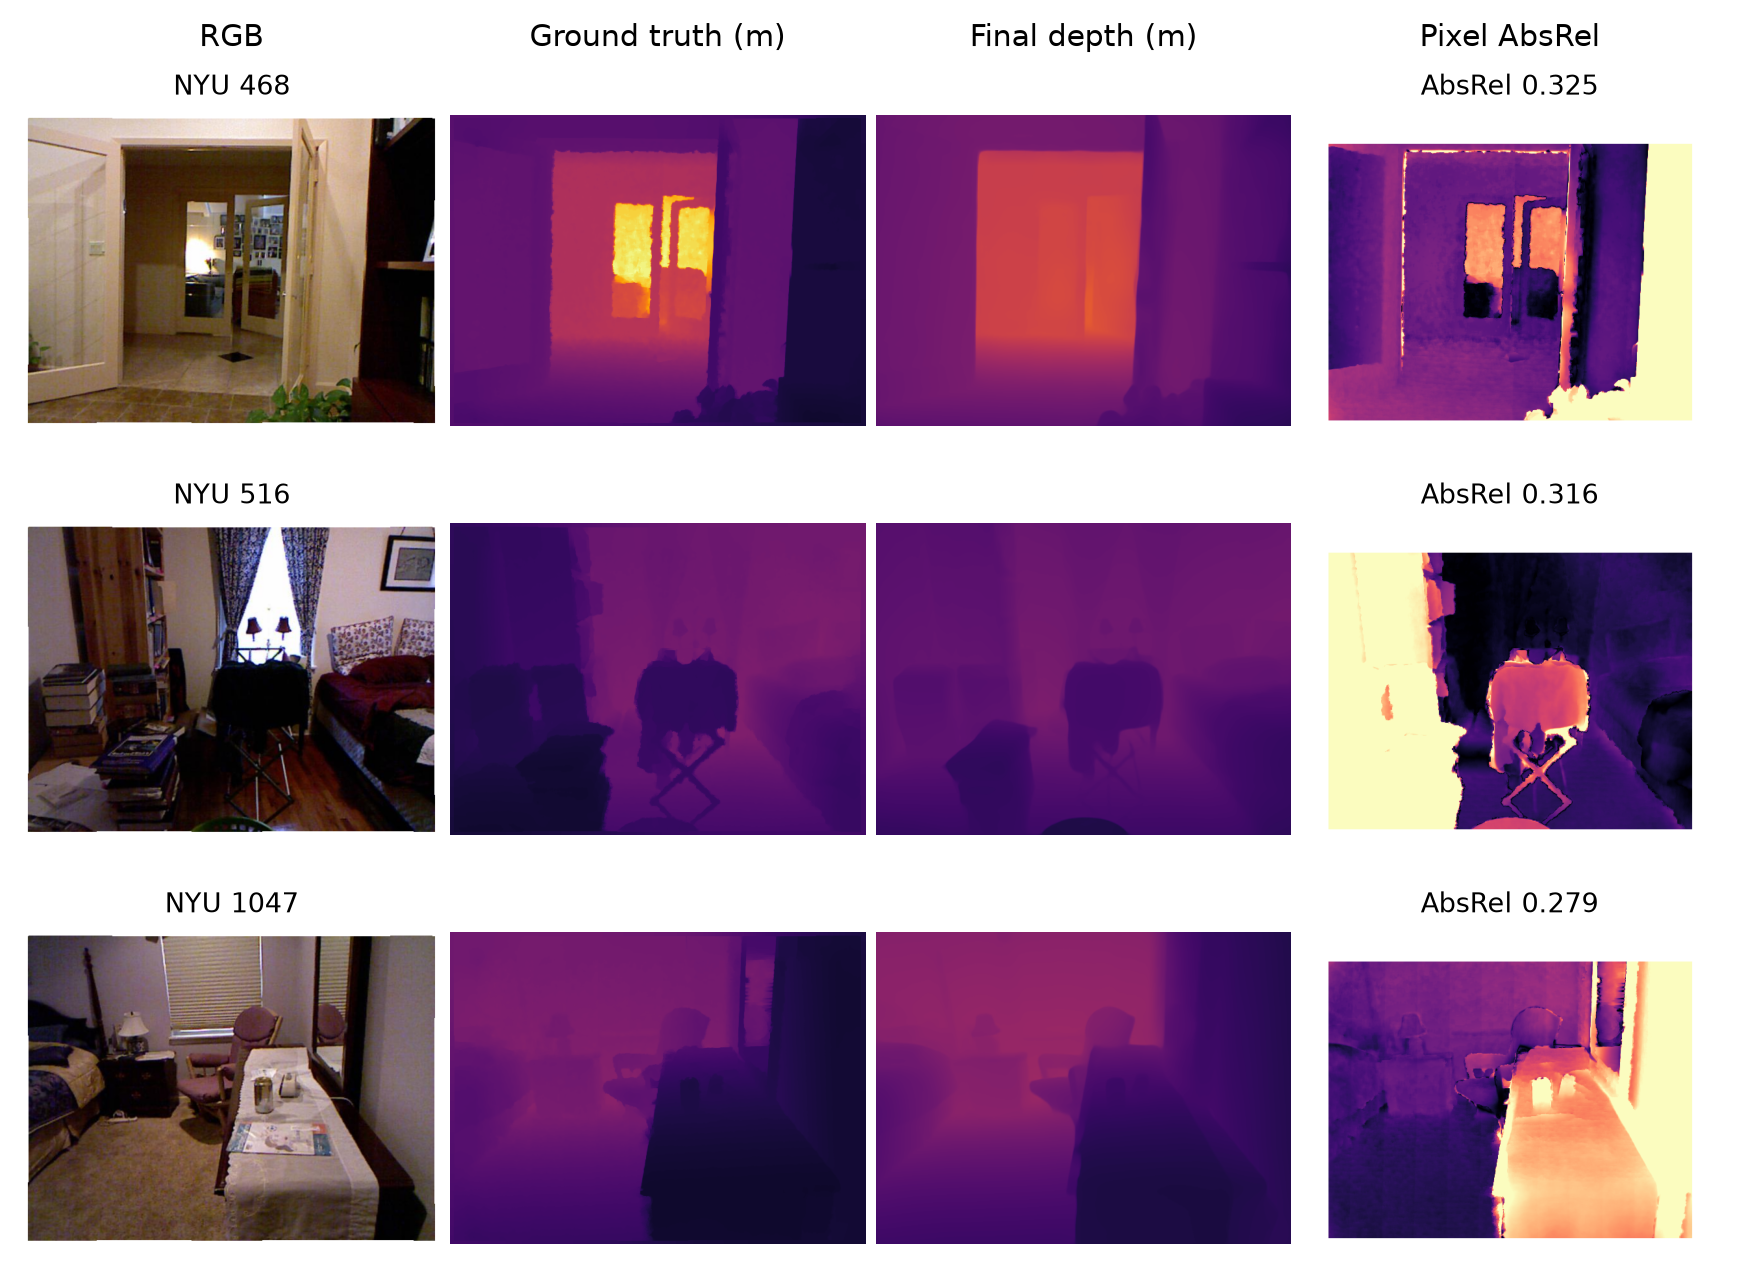
\includegraphics[width=.94\textwidth]{research-hard-cases.png}
\caption{Three actual hardest final-model test images, chosen by final AbsRel. Depth predictions share the GT 0--10 m display range. Error colors are capped at pixel AbsRel 0.5. Boundary and absolute-scale errors remain visible despite the aggregate gain.}
\label{fig:hard}
\end{figure*}
NYU 468 has final AbsRel 0.32490. The filled GT assigns large distances to the bright rear rectangles, while the prediction compresses this depth variation. Error also concentrates along the near right-hand boundary. NYU 516 reaches 0.31564, with disagreement on the dark chair, its thin crossed legs, and the left foreground stacks against a bright window. NYU 1047 reaches 0.27923, with large proportional error over the near table and right-hand mirror region. The predicted tabletop and chair boundaries are smoother than the GT geometry.

The largest individual regression is the narrow bookstore aisle in NYU 85. AbsRel rises from 0.08101 to 0.19892, with error spread over the shelving surfaces. The largest gain is the study room in NYU 278, where AbsRel falls from 0.36117 to 0.08131. Its raw prediction places much of the rear interior too far away. The median-change example, NYU 1021, changes from 0.09043 to 0.06585.

NYU filled depth combines Kinect measurements with filled regions. Missing measurements, reflections, and mixed boundary pixels limit interpretation of local errors. The adapter can also learn indoor scene priors from the development distribution. Performance on other cameras, outdoor images, and video remains unmeasured.

\subsection{Mandatory Stereo Exercise}
OpenCV fixed-point disparity $r$ is converted to pixels by $d=r/16$. With focal length $f$, baseline $B$ in millimeters, and calibration offset, depth in meters is
\begin{equation}
z=\frac{fB}{d+\mathrm{doffs}}\frac{1}{1000}.
\end{equation}
For $r=160$, $f=1000$, $B=100$, and $\mathrm{doffs}=2$, this gives $d=10$ px and $z=8.333$ m. We use the quarter-resolution calibration and mask invalid disparities.

SGBM uses block size 5, $P_1=200$, $P_2=800$, uniqueness 10, speckle window 100, and 3WAY mode. The disparity range is rounded up from calibration to a multiple of 16. Across all 15 pairs, mean pair MAE is \StereoMAE{} px and mean coverage is \StereoCoverage\%. MAE uses positive finite prediction/GT intersection, while coverage divides by all valid GT pixels.

\begin{figure*}[t]
\centering
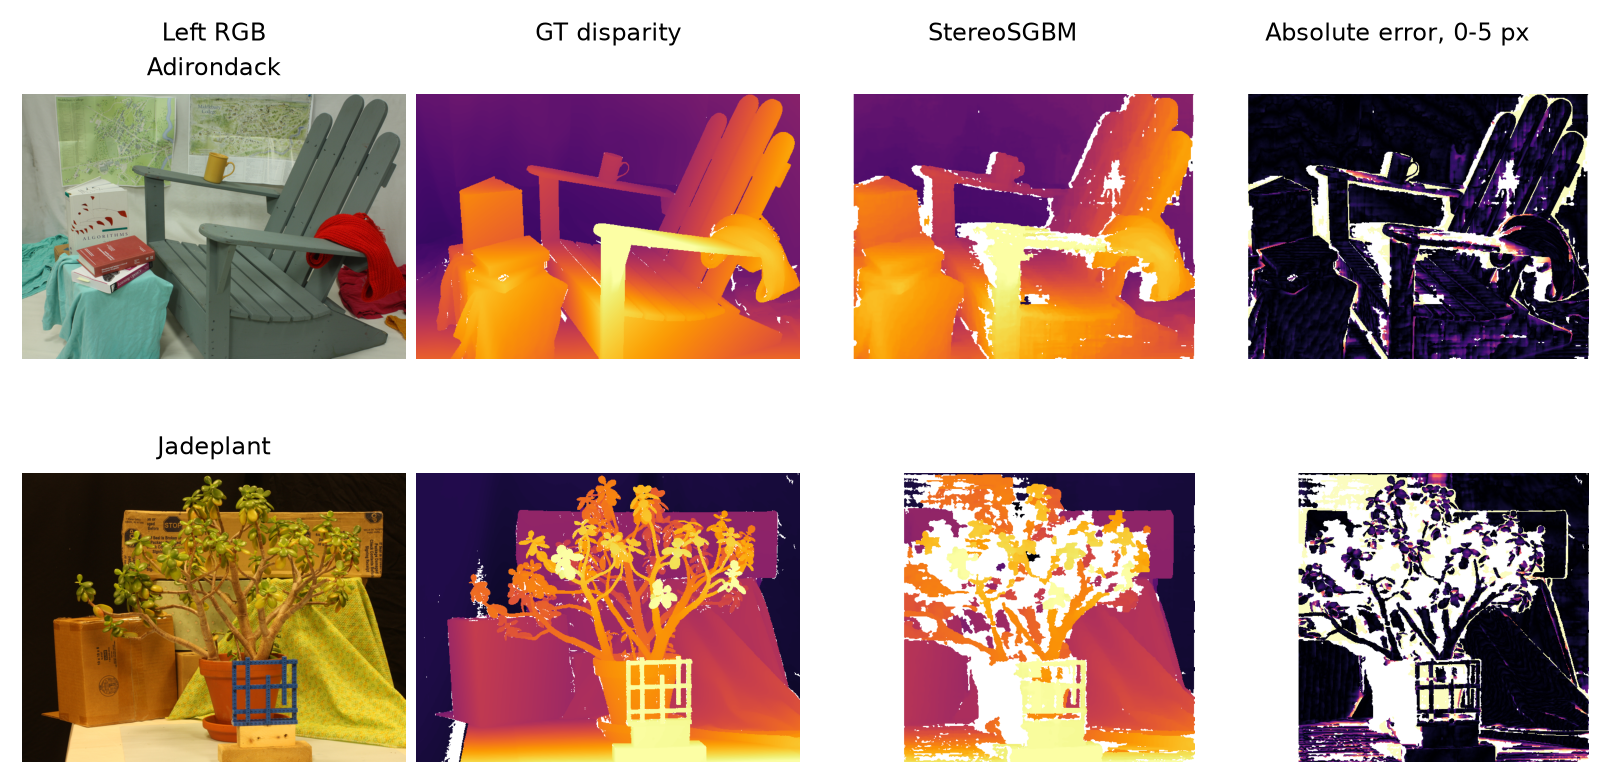
\includegraphics[width=.9\textwidth]{stereo-comparison.png}
\caption{Calibrated SGBM on Adirondack and Jadeplant. Disparity ranges are shared within each pair, invalid estimates are masked, and error display is capped at 5 px. Thin structures and occlusions remain difficult.}
\end{figure*}

\subsection{Required Relative-Video Comparison}
DA V2-Small runs independently per frame with input size 518. VDA-Small runs offline FP16 with input size 392 after the allowed memory reduction. Both use the same genuine source frames. Each method has a fixed whole-clip 2nd/98th-percentile normalization with a shared palette. Equal colors across methods have no common distance in meters.

\begin{figure*}[t]
\centering
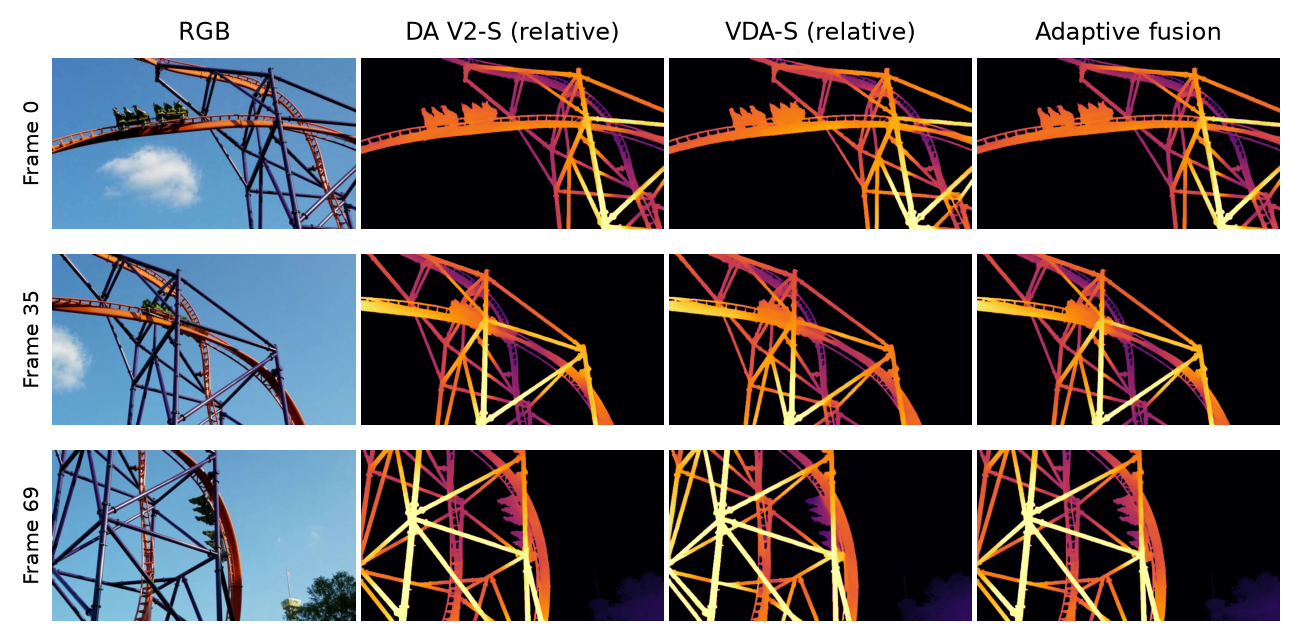
\includegraphics[width=\textwidth]{video-comparison.png}
\caption{Genuine frames 0, 35, and 69 for the required RGB/DA V2/VDA comparison. The fourth column retains the earlier temporal-fusion experiment. Each method preserves fixed clip-wide normalization and chronological source content.}
\end{figure*}

The models recover the large track structure, with remaining changes around supports and moving boundaries. The earlier flow-guided fusion changed predictions by only 0.22\% of the fixed display range on average, explaining its subtle visible effect. Its 18.23\% stability-proxy gain measures a chosen temporal-change statistic. The clip has no supplied true depth, so this statistic cannot establish metric-depth accuracy. The final accuracy comparison uses the separate NYU ground truth.

\subsection{Runtime and Application}
\begin{table}[t]
\centering\small
\caption{Isolated RGB-to-depth inference. Memory columns are peak allocated (A) and reserved (R) MiB.}
\begin{tabular}{lrrr}
\toprule
Method & ms/img & A & R\\
\midrule
Raw, default & 37.4 & 486 & 604\\
Raw, resolution 4 & 36.8 & 537 & 692\\
Raw, resolution 9 & 47.6 & 715 & 942\\
Previous refiner & 84.5 & 500 & 606\\
Selected (577 fit) & 326.6 & 438 & 564\\
Final (795 fit) & 235.8 & 438 & 564\\
\bottomrule
\end{tabular}
\end{table}

The three final all-development refits take 7,190 s in total, with maximum peak allocated memory 3,447 MiB. This duration includes epoch-loop training, fitting-score passes, checkpoint writes, and the final reload check. Model and data setup are excluded. AdamW, gradient-scaler, optimizer, and RNG states are retained for resumption.

The isolated benchmark uses an RTX 4070 Laptop GPU with 8,188 MiB VRAM, PyTorch 2.8.0/CUDA 12.8, FP16 foundation inference, 30 development images from different scenes, two warmups, and three repeats. Each timed call covers CPU RGB to CPU metric depth, including preprocessing, all model passes, refinement or seed averaging, and postprocessing. GPU synchronization brackets calls. File I/O, metrics, and compression are excluded.

The raw reference median is \ResearchBaseMS{} ms/image and final median is \ResearchFinalMS{} ms/image. Peak allocated/reserved memory is reported separately for each method. Larger-input references use the same real adapter entry point, with actual internal dimensions recorded. Training runs are stopped during the benchmark.

\begin{figure*}[t]
\centering
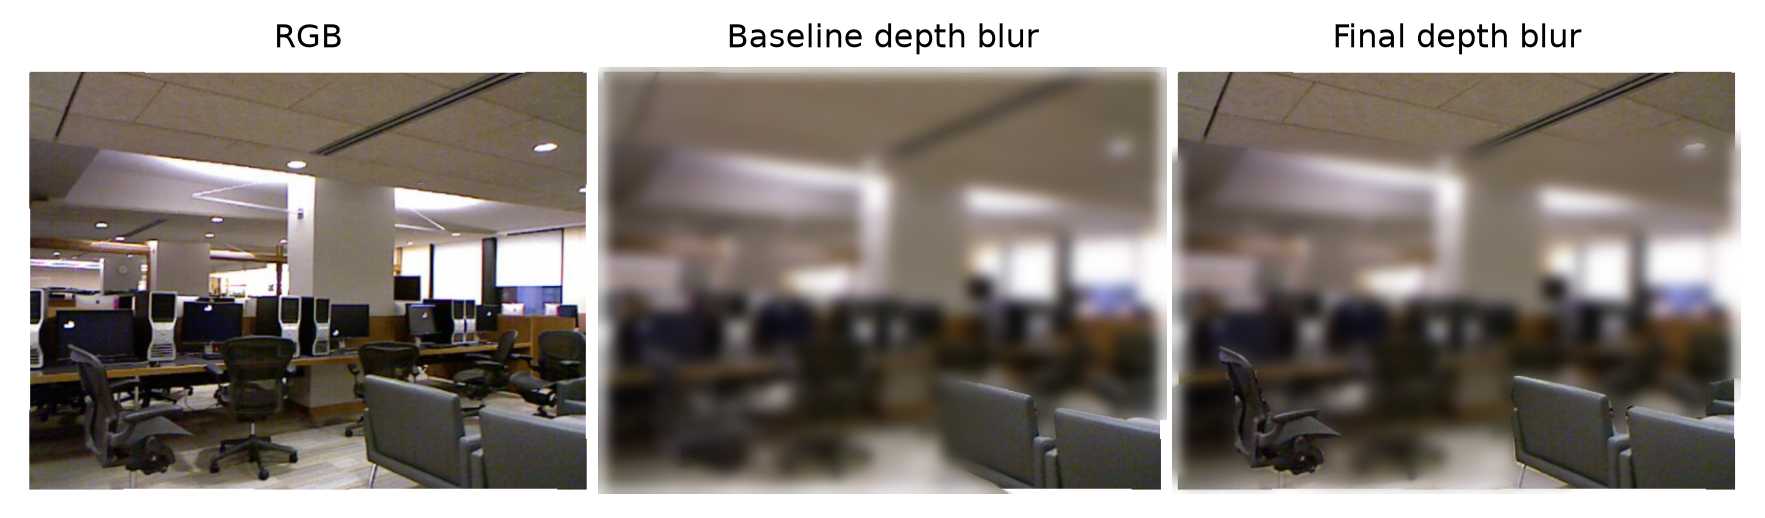
\includegraphics[width=\textwidth]{research-application.png}
\caption{Depth-based background blur using identical RGB, 3 m focus threshold, 0.4 m transition, and Gaussian blur. The manually chosen focus setting is fixed across the baseline and final prediction. The example follows the largest-gain image rule.}
\end{figure*}

VDA's reduced input run takes 6.94 s for 70 frames and reports 3,072/4,194 MiB allocated/reserved, compared with 73.49 s and 8,014/11,858 MiB at input 518. These are earlier recorded video-run measurements. Logical CUDA counters under Windows do not establish physical residency by themselves.

\section{Reproducibility and Limitations}
The implementation occupies an independent directory on an experiment branch. Foundation weights and data remain external. The small learned adapter weights, frozen recipe, data identities, source hashes, selection results, per-image test CSVs, and benchmark summaries accompany the report. Raw float prediction packets support independent metric recomputation. An independent NumPy implementation recomputes all 654-image metrics with maximum difference $1.9\times10^{-15}$. Raw-reference and previous-refiner pixels exactly match their preserved test packets. The final recipe and weights are committed before new test inference.

The original baseline and previous refiner test outcomes had already been inspected before this new study. The new selection search uses development images, but the reported result inherits that prior test-history exposure. The scene bootstrap omits search uncertainty, and three seeds provide a limited estimate of training variability. Additional supervision and inference passes change the operating setting relative to the original pretrained reference. The final all-development refit is retained according to its predeclared rule even if a test metric regresses.

The source video supplies 70 frames, and the archive records this limit. The report retains a draft author line for group confirmation. Model code, pretrained sources, papers, dataset sources, and CVPR template remain attributed.

\section{Discussion}
The methods address different sources of prediction error. A global multiplier corrects a systematic distance bias shared across images. LoRA changes the internal representation through small learned attention updates, allowing the model to adapt to the NYU indoor distribution. The feature-guided refiner instead learns spatial corrections from RGB and frozen geometric features. These are hypotheses about useful mechanisms, evaluated through their complete prediction pipelines.

On the same 218 selection images, the native-feature refiner has three-seed mean AbsRel 0.09336 and rank-8 high-rate LoRA has 0.08740. The development data-size curve concerns the earlier residual architecture, so its saturation provides motivation for changing the adaptation mechanism. It does not establish a universal data requirement for every model family.

Flip averaging tests sensitivity to an equivalent image view. Horizontal mirroring preserves the scene's distances, and restoring output coordinates permits pixelwise fusion. In a simplified example, a surface at 3 m receives predictions 2.7 m and 3.1 m from the original and restored-flip views. The fixed 75/25 blend gives 2.8 m, reducing its proportional error from 10\% to 6.7\%. The actual benefit is measured across held-out images, since correlated or systematically wrong predictions can also reinforce errors.

Across the three trained LoRA seeds, fixed flip averaging changes mean single-seed selection AbsRel from 0.08740 to 0.08630. Averaging the three seed predictions then gives 0.08525, compared with 0.08548 for the median-scoring individual seed. The latter comparison evaluates prediction averaging, while the three-seed mean evaluates the training recipe. The two statistics answer different selection questions.

The supported thesis is that a small amount of supervised adaptation plus fixed view/seed averaging improves this reproduced metric-depth reference on NYU. The raw reference and final model share the same test images, units, crop, and metric arithmetic. Development labels and additional inference passes are explicit parts of the improvement. Detailed claims about boundary accuracy, calibration transfer, or other datasets require their own measurements.

\section{Conclusion}
The selected \ResearchMethod{} yields test AbsRel \ResearchFinalAbs{} under the course's metric-depth protocol, a \ResearchGain\% reduction against reproduced UniDepthV2-S. Scene-separated comparisons, repeated seeds, and a fixed all-development refit make the selection path reproducible. Shared-scale GT error figures and per-image regressions qualify the aggregate result. Required stereo, relative-video comparison, and the depth application remain included with their units and source limitations.
\clearpage
\twocolumn
{\small
\bibliographystyle{ieeenat_fullname}
\bibliography{references,metric-research-references}
}
\end{document}
